\documentclass[dvipdfmx]{jarticle}
\usepackage{graphicx}
\usepackage{here}
\usepackage{ascmac}
\usepackage{amsmath,amssymb}
\usepackage[margin=20mm]{geometry}
\usepackage{listings,jvlisting} %日本語のコメントアウトをする場合jvlisting(もしくはjlisting)が必要
%ここからソースコードの表示に関する設定
\lstset{
  basicstyle={\ttfamily},
  identifierstyle={\small},
  commentstyle={\smallitshape},
  keywordstyle={\small\bfseries},
  ndkeywordstyle={\small},
  stringstyle={\small\ttfamily},
  frame={tb},
  breaklines=true,
  columns=[l]{fullflexible},
  numbers=left,
  xrightmargin=0zw,
  xleftmargin=3zw,
  numberstyle={\scriptsize},
  stepnumber=1,
  numbersep=1zw,
  lineskip=-0.5ex
}
\setcounter{tocdepth}{4}
\pagestyle{empty}
\begin{document}
\title{計算機科学実験及演習4 データベース 課題1}
\author{1029-32-6611 山田裕晃}
\maketitle

\section{目的}
実験4にて作成するアプリケーション及びデータベースの概念設計を行う。

\section{課題内容}
\subsection{アプリケーションの説明}
イベントの予約を行うアプリケーションを作成する。

\subsection{利用者の役割の列挙と説明}
以下に挙げる役割を想定している。
\begin{description}
    \item[参加者] イベントの一般参加者。
    \item[主催者] イベントの主催者。 
    \item[スタッフ] イベント当日のスタッフ。
\end{description}

\subsection{役割ごとの機能の列挙と説明}
\begin{itemize}
    \item 参加者
    \begin{description}
        \item[イベントの予約] 定員に空きがあれば、参加したいイベントに申し込むことができる。
        \item[チケットの表示] QRコードを表示させる。
    \end{description}
    \item 主催者
    \begin{description}
        \item[イベントの登録] 新たにイベントを開催したい場合、イベントを登録できる。
        \item[イベント情報の設定] イベントの開催場所・定員などの情報を編集できる。
        \item[予約状況の確認] 定員に対する予約状況などを確認できる。
    \end{description}
    \item スタッフ
    \begin{description}
        \item[チケットの受付] チケットに表示されたQRコードを読み込むことで受付できる。
    \end{description}
\end{itemize}

\subsection{実体関連図とその説明(各実体集合および関連集合の説明)}

\begin{figure}[H]
    \centering
    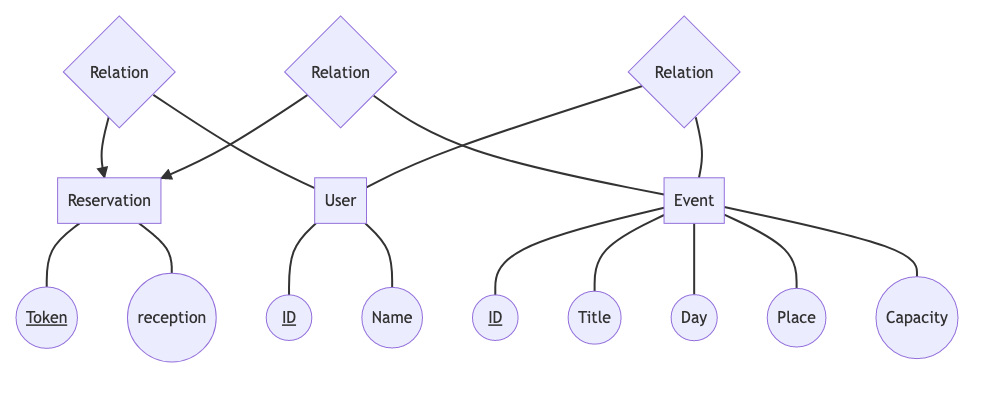
\includegraphics[scale=0.5]{ermodel.png}
    \caption{Compilation Report}
\end{figure}

\end{document}